\documentclass[UTF8]{ctexart}
\usepackage{graphicx}
\title{第一周周练题解}
\author{ZeNgBi}
\date{}
\begin{document}
	\maketitle
	\subsection*{P1000.apple}
	10个数字 暴力计数即可
	\subsection*{P1001.gloves}
	按照题意,每次配对最左边的手套。
	
	考虑暴力,每次从i+1处搜索另一个颜色相同的手套,然后逐个搜索,如果碰到已经配对成功的手套(vis[i]==true) 则continue本次循环 否则step++ 答案为$\sum$step 时间复杂度$O(n^2)$
	\subsection*{P1002.acwk}
	纯模拟题 需要两个数组 trans[],vis[],trans表示翻译结果 比如trans[1]=2 表示A翻译成B,vis表示哪些密字已经使用过。
	
	然后暴力破译,在破译过程中如果遇到trans[a[i]]已经赋值 或者vis[b[i]]已经被使用 则出现矛盾 破译失败
	
	翻译过程中如果trans[c[i]]还没有赋过值 则破译失败 否则依次输出trans[c[i]]
	
	(以上a[i],b[i],c[i]表示输入的第一行第二行第三行,其中的字符'A'-'Z'用数字1-26表示)
	\subsection*{P1003.power}
	暴力计算有多少个普通点和特殊点,那种点多哪边赢,相同则平局
	\subsection*{P1004.robot}
	只要有一边的方向上有障碍物就可以对着这面墙疯狂摩擦,保证安全,输出-1
	如果四个方向都没有障碍物,假设当前位置为(x,y)那么最多向左走x-1步,或者向右走m-x步,向上走n-y步或者向下走y-1步,如果在四个方向上多出一个命令都会导致不安全,可以证明答案为m+n-2
	\subsection*{P1005.table}
	要使涂完之后的地毯看上去是由一块一块矩阵构成的,那么我们就得保证上一行的图形与这一行的图形完全相同或者完全相反。列同理。
	\begin{figure}[!htb]
		\centering
		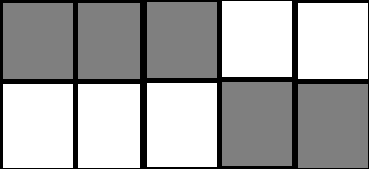
\includegraphics[height=0.1\textheight,width=0.4\textwidth]{p10051}
		\caption{正确情况}
	\end{figure}
	\begin{figure}[!htb]
		\centering
		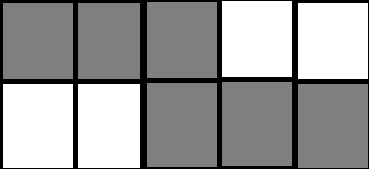
\includegraphics[height=0.1\textheight,width=0.4\textwidth]{p10052}
		\caption{错误情况}
	\end{figure}
	
	这就说明我们需要一个模板来控制每一行的颜色,容易想到暴力枚举每种模板,然后行列各一次,计算最小需要涂色的格子数量,但是这样仅仅是枚举的时间复杂度就有O($2^n$)是肯定是不能过掉这个题的。
	
	这个时候需要更高效的枚举方式,于是我选择用现有的每一行做模板进行计算,列同理(原理未知),最后发现极端数据:
	
	5 5 10
	
	1 0 0 0 0 
	
	0 1 0 0 0
	
	0 0 1 0 0 
	
	0 0 0 1 0
	
	0 0 0 0 1
	
	针对这种数据只需拿空白模板(全为0或者全为1的模板)进行计算就好(原理同样未知)
	
	时间复杂度O($n^3$)
	
\end{document}